\subsection{MOSFET Threshold Voltage}
 The first part of this analysis was to determine the values of $I_{DS}$ and $\sqrt{I{DS}}$ and put them into a table which is below.
 
 \begin{table}[h]
    \begin{tabular}{@{}cccccc@{}}
\toprule
\textbf{$V_{BB}$ (V)} & \multicolumn{1}{l}{\textbf{$V_{GG}$ (V)}} & \textbf{$V_{DD}$ (V)} & \textbf{$V_{DS}$ (V)} & \textbf{$I_{DS}$} & \textbf{$\sqrt{I_{DS}}$} \\ \midrule
%                        VGG     VDD     VDS     IDS  sqrt(IDS)
\textit{\textbf{0}}     &  2.86     &   7.09    &  6.0550     & 1.0108    & 1.0054 \\
\textit{\textbf{0}}     &  3.60     &   8.15    &  6.0768       &  2.0041  & 1.4157    \\
\textit{\textbf{0}}     &  4.22     &   9.13    &  6.0277     & 3.0031      & 1.7329\\
\textit{\textbf{0}}     &  4.76     &   10.17    & 6.0273      & 4.0049     & 2.0012\\
\textit{\textbf{0}}     &  5.27     &   11.21    & 6.0167       &   5.0176   & 2.24\\ \bottomrule
\end{tabular}
    \caption{MOSFET characteristics at $V_{BB}$ = 0}
    \label{tab:VBB0L}
\end{table}

\begin{table}[ht]
    \begin{tabular}{@{}cccccc@{}}
\toprule
\textbf{$V_{BB}$ (V)} & \multicolumn{1}{l}{\textbf{$V_{GG}$ (V)}} & \textbf{$V_{DD}$ (V)} & \textbf{$V_{DS}$ (V)} & \textbf{$I_{DS}$} & \textbf{$\sqrt{I_{DS}}$} \\ \midrule
%                        VGG     VDD     VDS     IDS  sqrt(IDS)
\textit{\textbf{-2}}     &  4.48     &  7.06     & 6.0200       &  1.0062    & 1.0031  \\
\textit{\textbf{-2}}     &  5.18     &  8.07     & 6.0013      &  2.0049     & 1.4159\\
\textit{\textbf{-2}}     &  5.75     &  9.12     & 6.0210  &    3.0004  & 1.7322\\
\textit{\textbf{-2}}     &  6.27     &  10.21     & 6.0476    & 4.0233  & 2.0058  \\
\textit{\textbf{-2}}     &  6.75     &  11.20     & 6.0050   & 5.0190   & 2.2403  \\ \bottomrule
\end{tabular}
    \caption{MOSFET characteristics at $V_{BB}$ = -2}
    \label{tab:VBB2L}
\end{table}

\begin{table}[ht]
    \begin{tabular}{@{}cccccc@{}}
\toprule
\textbf{$V_{BB}$ (V)} & \multicolumn{1}{l}{\textbf{$V_{GG}$ (V)}} & \textbf{$V_{DD}$ (V)} & \textbf{$V_{DS}$ (V)} & \textbf{$I_{DS}$} & \textbf{$\sqrt{I_{DS}}$} \\ \midrule
%                        VGG     VDD     VDS     IDS  sqrt(IDS)
\textit{\textbf{-6}}     &  6.64     & 7.05      & 6.0200      &1.0014   & 1.0006    \\
\textit{\textbf{-6}}     &  7.31     & 8.12      & 6.0434       & 2.0131 & 1.4188       \\
\textit{\textbf{-6}}     &  7.86     & 9.12      & 6.0099      & 3.0064  & 1.7339      \\
\textit{\textbf{-6}}     &  8.36     & 10.19      & 6.0380       & 4.0219 &2.0055       \\
\textit{\textbf{-6}}     &  8.81     & 11.22      & 6.0200      & 5.0171 & 2.2399      \\ \bottomrule
\end{tabular}
    \caption{MOSFET characteristics at $V_{BB}$ = -6}
    \label{tab:VBB6L}
\end{table}

\begin{table}[ht]
    \begin{tabular}{@{}cccccc@{}}
\toprule
\textbf{$V_{BB}$ (V)} & \multicolumn{1}{l}{\textbf{$V_{GG}$ (V)}} & \textbf{$V_{DD}$ (V)} & \textbf{$V_{DS}$ (V)} & \textbf{$I_{DS}$} & \textbf{$\sqrt{I_{DS}}$} \\ \midrule
%                        VGG     VDD     VDS     IDS  sqrt(IDS)
\textit{\textbf{-10}}     & 8.28      & 7.05      & 6.0195      & 1.0019   & 1.0009   \\
\textit{\textbf{-10}}     & 8.93      & 8.14      & 6.0714      & 2.0046   & 1.4158      \\
\textit{\textbf{-10}}     & 9.48      & 9.16      & 6.0354       & 3.0200  & 1.7378   \\
\textit{\textbf{-10}}     & 9.96      & 10.19      & 6.0191      & 4.0268  & 2.0067    \\
\textit{\textbf{-10}}     & 10.41      &  11.21     &  6.0154     & 5.0133 & 2.2349     \\ \bottomrule
\end{tabular}
    \caption{MOSFET characteristics at $V_{BB}$ = -10}
    \label{tab:VBB10L}
\end{table}

From the data given we then plotted the values $\sqrt{I_{DS}}$ vs $V{GS}$ and drew a line of best fit on each of the plot point. The line was then extrapolated to 0 for us to determine the threshold voltage $V_T$.\\

\begin{figure}[ht]
    \centering
    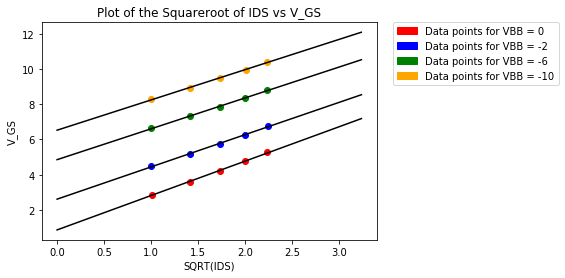
\includegraphics[width=.96\linewidth]{figures/threshold_voltage_plot.png}
    \caption{The plot of $\sqrt{I_{DS}}$ vs $V{GS}$}
    \label{fig:thershold}
\end{figure}
From the graphs we were able to determine the threshold voltage $V_T$ for each $V_{BS}$. 

\begin{table}[ht]
    \begin{tabular}{@{}cc@{}}
    \toprule
    \textbf{$V_{T}$ (V)} & \textbf{$V_{BS}$ (V)} \\ \midrule
    0.867 &         0           \\
    2.61  &        -2           \\
    4.85  &        -6          \\
    6.53  &        -10                   \\
 \bottomrule
\end{tabular}
    \caption{Voltage Threshold at each $V_{BB}$}
    \label{tab:VT}
\end{table}
As we can see the value of $V_t$ when $V_{BB} = 0$ is 0.867V, which is different to the value of $V_T$ that we found in the previous part during the experiment which is 1.58V.From this data we then plotted $V_T$ vs $V_{BS}$, and drew a curve through the points.\\
\begin{figure}[ht]
    \begin{subfigure}[b]{0.40\linewidth}
    \centering
    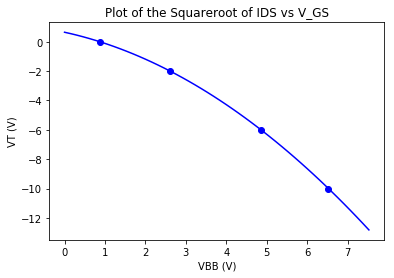
\includegraphics[width=0.95\linewidth]{figures/VT_vs_VBB.png}
    \caption{The plot of $V_t$ vs $V{BS}$}
    \label{fig:thers}
    \end{subfigure}
    \begin{subfigure}[b]{0.40\linewidth}
    \centering
    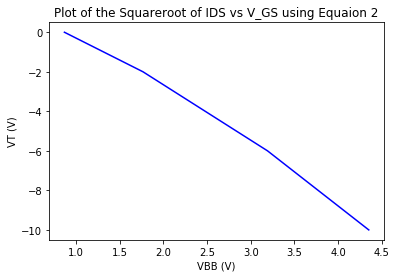
\includegraphics[width=0.95\linewidth]{figures/VT_vs_VBB_EQ2.png}
    \caption{The plot of Equation 2}
    \label{fig:EQ2}
    \end{subfigure}
\end{figure}
From the figure above we can see that the shape of the curve that we plotted with the data we obtained matched that of the shape of the curve that is created with equation 2 in the lab manual. The only difference would depend on the model parameters $\gamma$ and $\phi$.\\
\begin{equation}
    I_{DS} = K(V_{GS} - V_T)^2 
\end{equation}

Is equation 1, from this we know that $\sqrt{K}$ is the slope of the lines in Figure \ref{fig:thershold} we can see that the non-zero values of $V_{BS}$ do not really effect the K parameter. The only thing that is effected is the threshold voltage $V_T$.
\clearpage
\subsection{Semiconductor Parameter Analyzer}

\subsubsection{\texorpdfstring{$I_{DS}$ vs. $V_{DS}$ Characteristics for various $V_{GS}$}{Dump to Source Current vs Voltage Characteristics for various Gate to Source Voltages}}

First we will look at the MOSFET's three terminal characteristics:

\begin{figure}[ht]
    \centering
    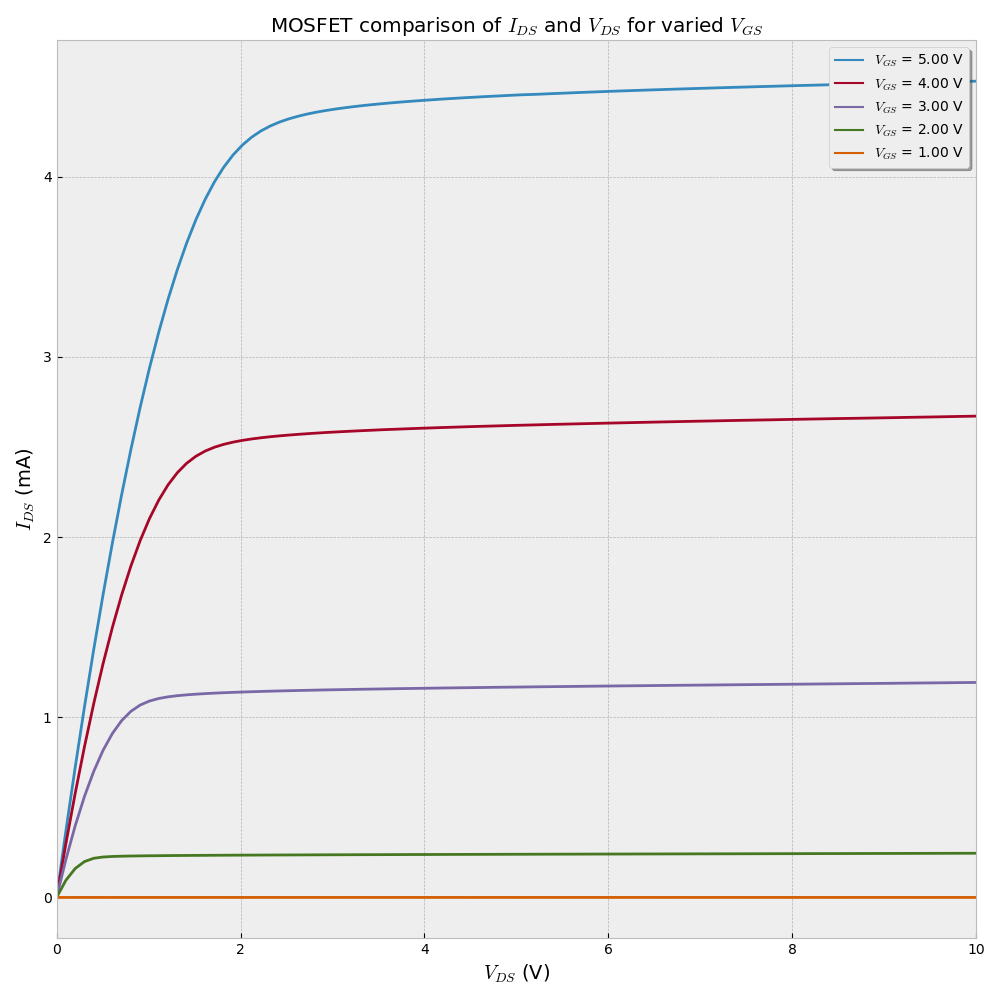
\includegraphics[width=.95\linewidth]{figures/characteristic_nothing.png}
    \caption{The characteristic graphs of $I_{DS}$ vs. $V_{DS}$ for several differing values of $V_{GS}$. }
    \label{fig:characteristic}
\end{figure}

\clearpage

We also view these three terminal characteristics through the Agilent Software, which is shown here:

\begin{figure}[ht]
    \centering
    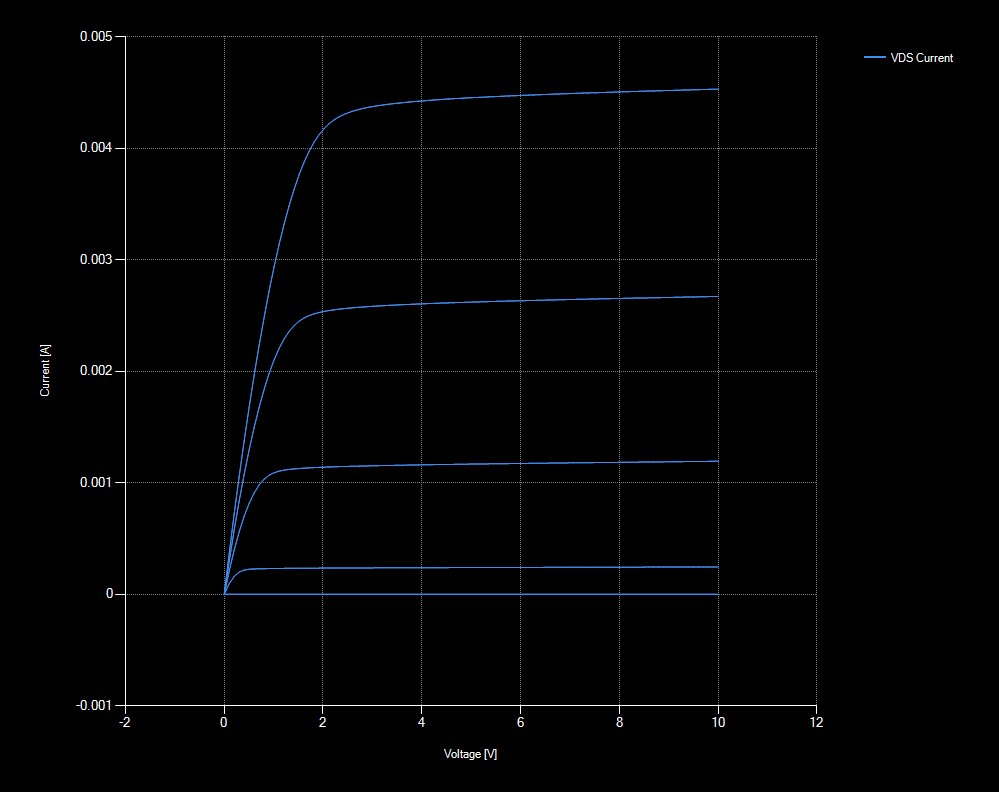
\includegraphics[width=.95\linewidth]{figures/ECE331_Lab3_Data421V1}
    \caption{The characteristic graphs of $I_{DS}$ vs. $V_{DS}$ for several differing values of $V_{GS}$. Shown with in-lab software }
    \label{fig:characteristic_inlab}
\end{figure}

From these graphs we can calculate two important characteristics, these are the MOSFET output resistance $r_o$ and the trans conductance $g_m$.

We note that we can calculate the output resistance by taking two points along a single $V_{GS}$ (The points taken are shown in Figure \ref{fig:VGS_varied}) through $r_o = ( \frac{\partial I_{DS}}{\partial V_{DS}}|_{V_{GS} = constant}$)$^{-1}$. We simply use the delta between the markers where $\Delta V_{DS} \,= \,3.23\; V$  and $\Delta I_{DS} \,= \,75.77\;\mu A$ where $V_{GS}\, = \, 5.00 V$. Therefore $r_o \, = \, 42.63 \;k\Omega$.

We then calculate transconductance $g_m$, where this is defined as $g_m = \frac{\partial I_{DS}}{\partial V_{GS}}|_{V_{DS} = constant}$. The points taken are shown in Figure \ref{fig:VGS_constant}, where the deltas $\Delta V_{GS} \,= \,1.00\; V$  and $\Delta I_{DS} \,= \,1.815\;m A$ where $V_{DS}\, = \, 3.73 V$. Therefore $g_m \, = \, 1.815 \;mS$.

\clearpage

To find the early voltage, the saturation portion of the curves are fitted with a linear function and then the x intercept should be the value of the early voltage. The fitting is completed here, with the fit shown in  Figure \ref{fig:characteristic_tight_fit}. Then the intercepts are found in Figure \ref{fig:characteristic_wide_fit}. We see that there is large variation in the values of early voltage, leading to an experimentally found value of $V_E \, = \, -250 \pm 50 V$.

\begin{figure}[ht]
    \centering
    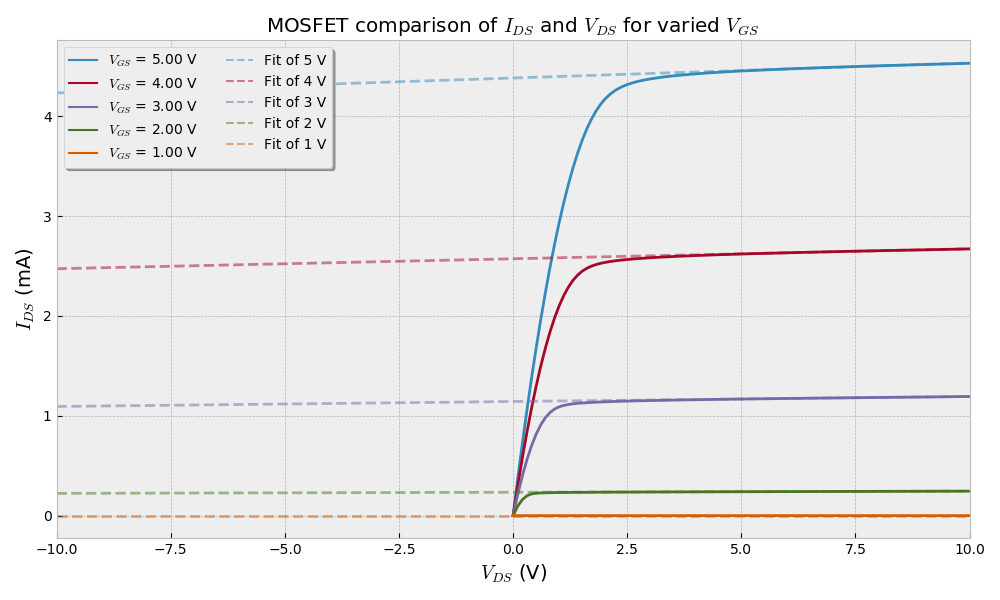
\includegraphics[width=.825\linewidth]{figures/characteristic_tight_fit.png}
    \caption{The characteristic graph with linear fit of saturation portion of curve to show quality of fit.}
    \label{fig:characteristic_tight_fit}
\end{figure}

\begin{figure}[ht]
    \centering
    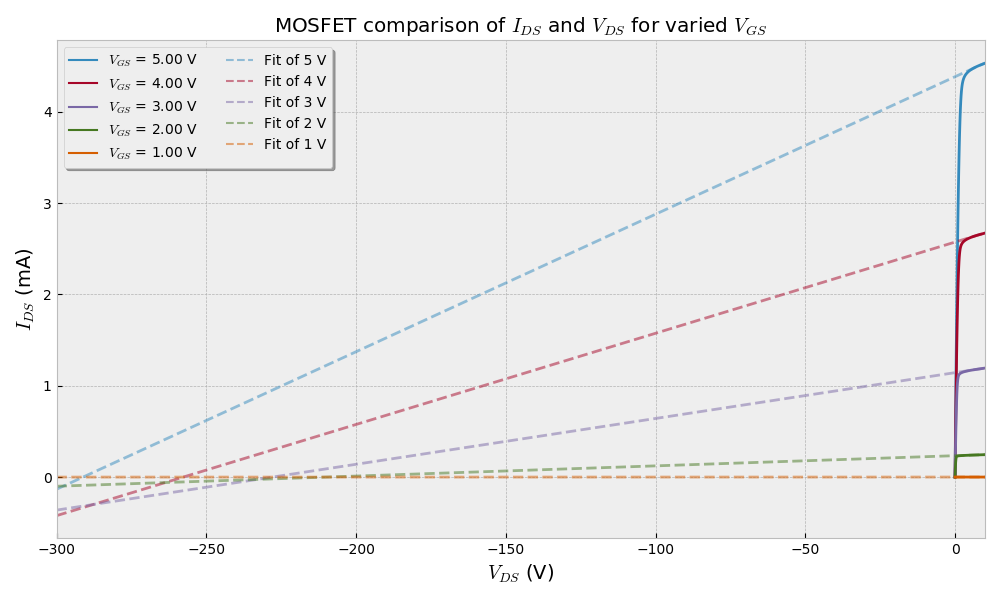
\includegraphics[width=.825\linewidth]{figures/characteristic_wide_fit.png}
    \caption{The characteristic graph with linear fit to show the Early Voltage}
    \label{fig:characteristic_wide_fit}
\end{figure}

\clearpage

To estimate the threshold voltage we graph the value of $I_{DS}$ vs. $V_{GS}$. this is shown in Figure \ref{fig:characteristic_threshold}. Due to the low number of $V_{GS}$ points which are taken, the determination of $V_T$ is a rough approximation. We approximate that it is 1V. This agrees with the found estimated value found during data collection and during part 1, A higher number of $V_{GS}$ points taken would allow for a more accurate approximation.

\begin{figure}[ht]
    \centering
    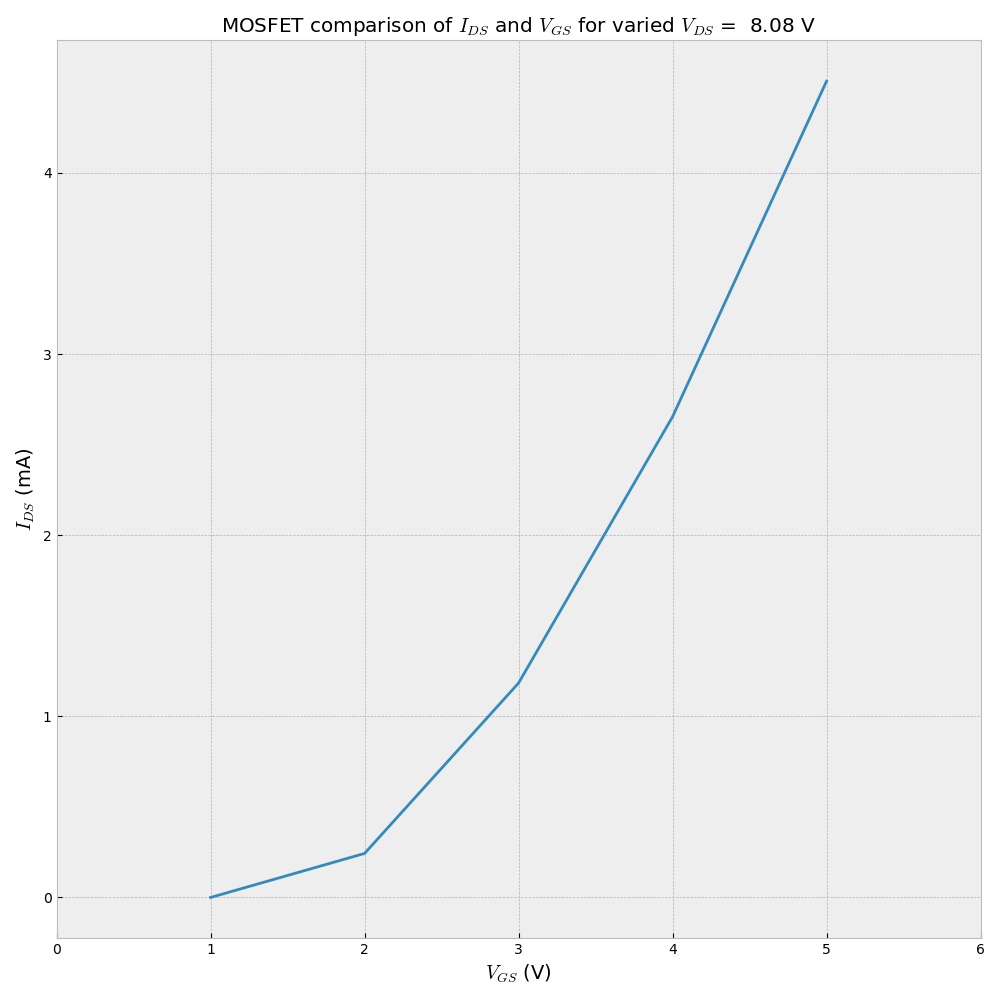
\includegraphics[width=.95\linewidth]{figures/characteristic_threshold.png}
    \caption{The characteristic graph of $I_{DS}$ vs. $V_{GS}$ used for determining the threshold voltage}
    \label{fig:characteristic_threshold}
\end{figure}

\clearpage

Finally for this characteristic graph we show the condition $V_{DS}$ = $V_{GS} - V_T$ which designates the two regions of the graph. These regions correspond to the triode region and the saturation region.

\begin{figure}[ht]
    \centering
    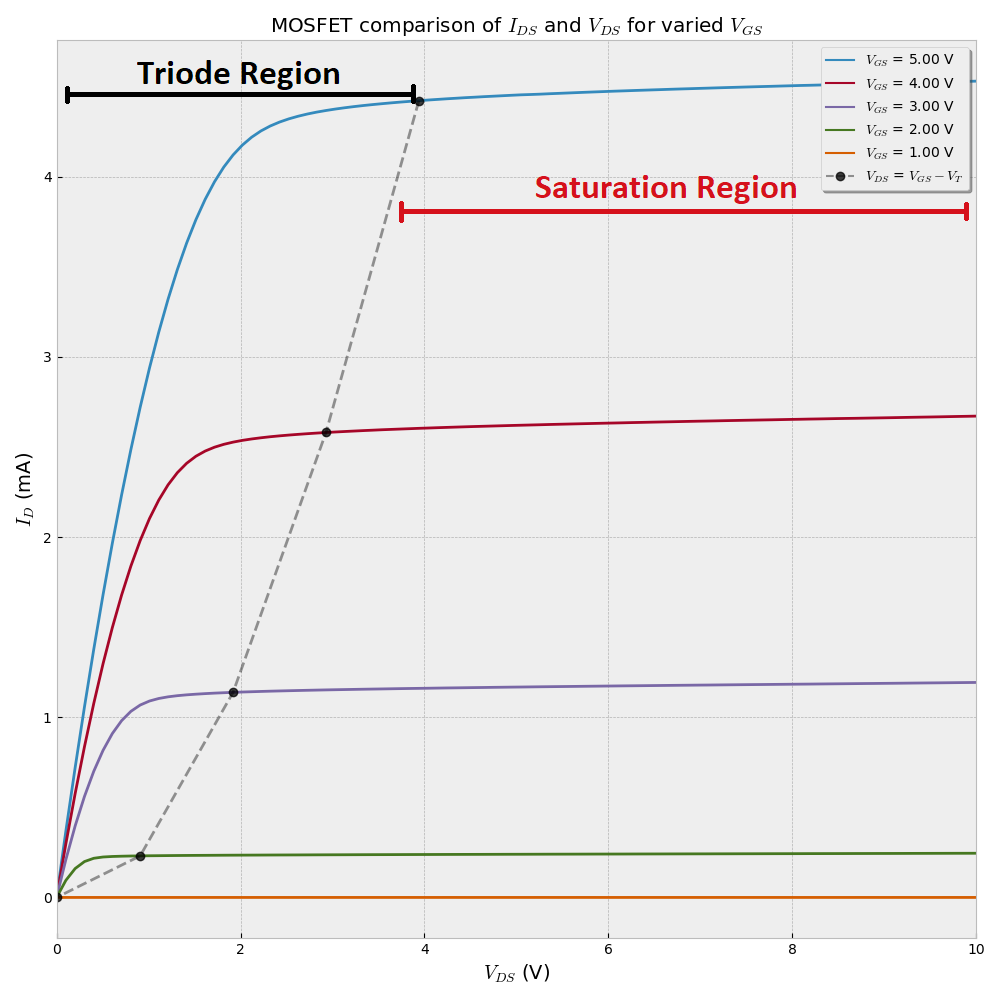
\includegraphics[width=.95\linewidth]{figures/characteristic_intercept_labelled.png}
    \caption{The characteristic graph of $I_{DS}$ vs. $V_{DS}$ with the condition $V_{DS}$ = $V_{GS} - V_T$ inputted and shown on graph}
    \label{fig:characteristic_intercept}
\end{figure}

\clearpage

\subsubsection{\texorpdfstring{$I_{DS}$ vs. $V_{DS}$ Characteristics for various $V_{GS}$ for small $V_{DS}$}{Dump to Source Current vs Small Voltage Characteristics for various Gate to Source Voltages}}

Here we take a look at the characteristic graph of $I_{DS}$ vs. $V_{DS}$ but for small positive and negative values of $V_{DS}$. This is shown in Figure \ref{fig:characteristic_small}. 

We also wish to determine if the MOSFET is behaving as a voltage controlled resistor. We note that a voltage controlled resistor will essentially behave as a passive resistor, except that a third terminal will be able to change the resistance of the device. We note that resistors are linear and in Figure \ref{fig:characteristic_small} we see that the slope of the curve and hence the resistance is controlled by the Gate Voltage. However we also note that the lines are not perfectly linear. These non-linear regions are evidence of distortion in the resistor. We conclude that the MOSFET can be used as a voltage controlled resistor, but care must be taken to avoid distortion effects.

\begin{figure}[ht]
    \centering
    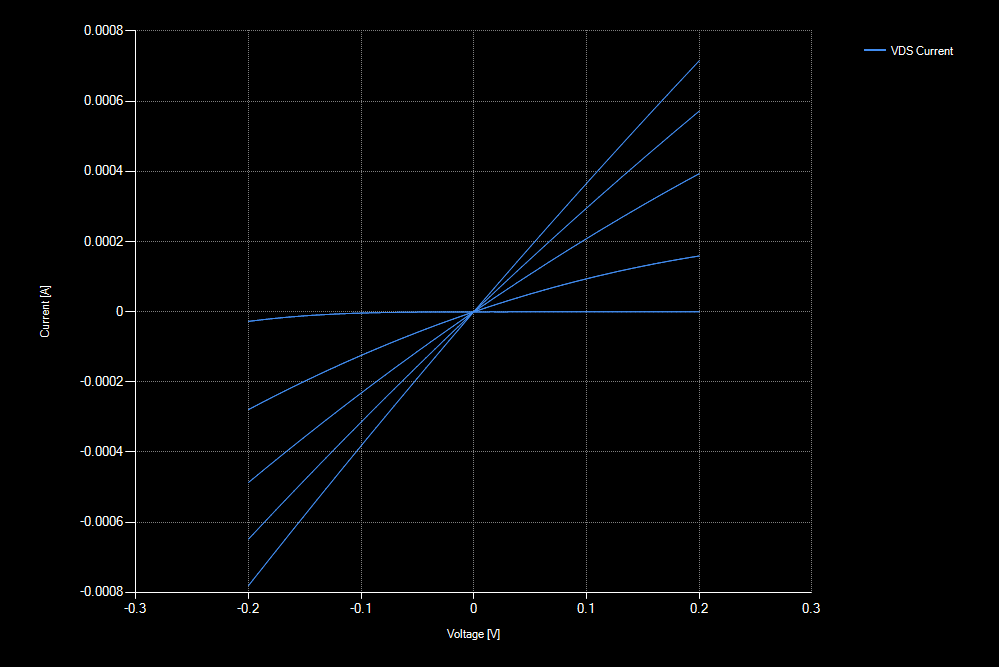
\includegraphics[width=.95\linewidth]{figures/ECE331_Lab3_Data422V1.png}
    \caption{The characteristic graph of $I_{DS}$ vs. $V_{DS}$ with small $V_{DS}$}
    \label{fig:characteristic_small}
\end{figure}